\section{Counting}
\subsection{Estimating distributions}
Estimating distributions is a practice in counting. Consider the election example in class. Let $y$ be the candidate an individual voter supports. Let $x_1, \ldots, x_n$ be the characteristics of each individual voter. These characteristics may include age, gender, race, party affiliation, etc. We want to estimate the distribution of $P(y | x_1, \ldots, x_n)$, the probability that a characterized individual supports a certain candidate. In an ideal world, we would obtain data from the entire population and represent the distribution perfectly. However, we are unable to do so when we are limited to small sample sizes of data. For example, if we consider 100 age groups, 2 genders, 5 races, and 3 parties, we need to form estimates across $100 * 2 * 5 * 3 = 3000$ groups. We are unlikely to obtain reliable estimates considering typical surveys collect on the order of 1000 responses.

\subsection{Solutions to data sparsity}
There are a few ways we can solve the data sparsity issue.\\\\
First, we can sacrifice the granularity of our estimates by binning our range of characteristic combinations into fewer groups. For example, instead of considering individuals of each age between 1 and 100 separately, we can consider individuals as part of groups between ages 1-18, 18-29, 30-49, etc.\\\\
We can also use more complex models that can be trained on small samples and generalize well. For example, instead of counting, we may choose a regression model.\\\\
Another solution is to obtain more data, estimate the relative frequencies in the problem, and use these relative frequencies. The data here should either be representative of the population or appropriately adjusted.

\subsection{Margin of error}
How many responses do we need to estimate $P(y)$ with a 5\% margin of error? The margin of error is equivalent to the standard error which is equivalent to the standard deviation in the sampling distribution of the mean. We used a Binomial random variable to represent the result of votes from $n$ individuals. Each time we simulate this random variable, we obtain an estimate of the true mean. Simulating this random variable many times yields an estimated distribution of the true mean. The standard deviation of this distribution is the margin of error.\\\\
We can also solve this problem by hand rather than through simulation. We represent each individual's vote as a Bernoulli random variable. Remember that $Var(X) = p(1-p)$ for a Bernoulli random variable $X$. We are looking for a relationship between the number of responses, $n$, the probability of voting for a certain candidate, $p$, and the margin of error, $s$. Note that $Var(\alpha X) = \alpha^2 Var(X)$ and $Var(X + Y) = Var(X) + Var(Y)$ if $X$ and $Y$ are independent.
$$Var\bigg(\frac{1}{n} \sum_{i=1}^n X_i\bigg) = \frac{1}{n^2}\sum_{i=1}^n Var\bigg(X_i\bigg), \ X_i \sim Bernoulli(p)$$
$$Var\bigg(\frac{1}{n} \sum_{i=1}^n X_i\bigg) = \frac{1}{n^2}\sum_{i=1}^n p(1-p)$$
$$Var\bigg(\frac{1}{n} \sum_{i=1}^n X_i\bigg) = \frac{np(1-p)}{n^2}$$
$$Var\bigg(\frac{1}{n} \sum_{i=1}^n X_i\bigg) = \frac{p(1-p)}{n}$$
$$s = \sqrt{\frac{p(1-p)}{n}}$$
$$n = \frac{p(1-p)}{s^2}$$
As in class, if $p = 0.5$ and $s = 0.05$, then we need $n = 100$ responses. Intuitively, if we want a smaller margin of error, we need more responses. If the probability becomes more fair and tends toward 50\%, we need more responses.

\subsection{Split, apply, combine}
The split, apply, combine method is useful for computing group statistics when all of the data can be loaded into memory. See Figure 1.
\begin{enumerate}
    \item Split or arrange all observations into their individual groups of interest
    \item Apply or compute distributions and statistics within each group of interest
    \item Combine or collect results across all groups of interest
\end{enumerate}
\begin{center}
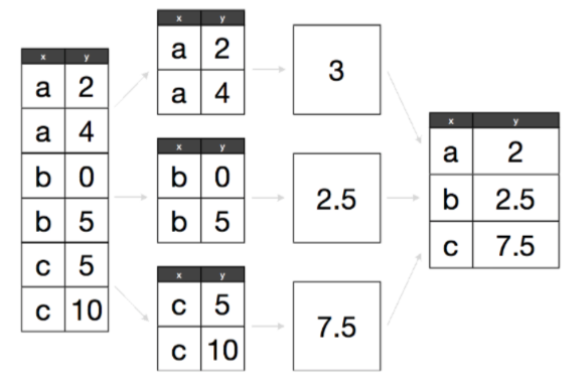
\includegraphics[width=0.4\linewidth]{figures/sac.png}\\
Figure 1. An example of the split, apply, combine method.
\end{center}

\subsection{Computing per group average}
Consider the following dataset. We wish to compute the average numerical value for each group, $A$, $B$, and $C$. Let $N$ be the number of observations and $G$ be the number of groups. Here, $N = 6$ and $G = 3$.
$$S = \{(A, 2), (A, 4), (B, 3), (B, 9), (C, 10), (C, 12)\}$$
The naive approach is to iterate through all observations, copy a list of values in group $A$, and iterate through all such group $A$ values to compute an average. Repeat this process for the remaining groups. This method takes $GN$ steps and $N$ space.\\\\
A better approach is to iterate through all observations, copy values of each group into separate lists, and compute an average for each list. This method takes $N$ steps and $N$ space.\\\\
The best approach is to iterate through each observation and keep a running sum and count of observations in each group. After all observations have been seen, compute the average for each group using the respective running sum and count. This method takes $N$ steps and $2G$ space.

\subsection{Computing per group variance}
Consider the dataset given previously. We now wish to compute the variance for each group. Define variance as $Var(X) = \frac{1}{n} \sum_{i=1}^n (x_i - \overline{x})^2$.\\\\
Note that the given formula requires that we know the average. The two pass method first passes through the data to compute per group average and then passes through the data again to compute per group variance.\\\\
We can simplify the formula for variance to develop a one pass method.
$$Var(X) = \frac{1}{n}\sum_{i=1}^n(x_i - \overline{x})^2$$
$$Var(X) = \frac{1}{n}\sum_{i=1}^n(x_i^2 - 2x_i\overline{x} + \overline{x}^2)$$
$$Var(X) = \frac{1}{n}\sum_{i=1}^nx_i^2 - \frac{2\overline{x}}{n}\sum_{i=1}^n x_i + \overline{x}^2$$
$$Var(X) = \frac{1}{n}\sum_{i=1}^nx_i^2 - 2\overline{x}^2\ + \overline{x}^2$$
$$Var(X) = \frac{1}{n}\sum_{i=1}^nx_i^2 - \overline{x}^2$$
However, note that for each value $x_i$, we compute $x_i^2$. This can cause value overflow, so this method should be avoided when working with large values.

\section{Anatomy of the long tail}
\subsection{Problem description}
The distribution of interests among individuals tends to exhibit a long tail. That is, there are few interests that are popular and many interests that are unpopular. The research paper presented in class attempts to answer where this long tail comes from on the subject of movies. Is it because some people only have mainstream interests while others only have niche interests? Or, does everyone have a blend of mainstream interests and niche interests with more variance among niche interests?

\subsection{Reading data at scale}
Large datasets may exceed available memory. Sampling may result in unreliable estimates for rare groups in the data. Randomly accessing data from disk is prohibitively slow. The best solution is to stream data. We read data one observation at a time and only store the state or values we require to calculate the statistics we are interested in.

\subsection{Distribution of the data}
Each entry in the dataset includes a user identifier, a movie identifier, and a rating. Thus, in order to compute statistics about each movie/rating, we first have to group entries by movie/rating. We compute these per group statistics using the methods we previously outlined. The data shows that most ratings, regardless of value, are given to the most popular movies. See Figure 2.
\begin{center}
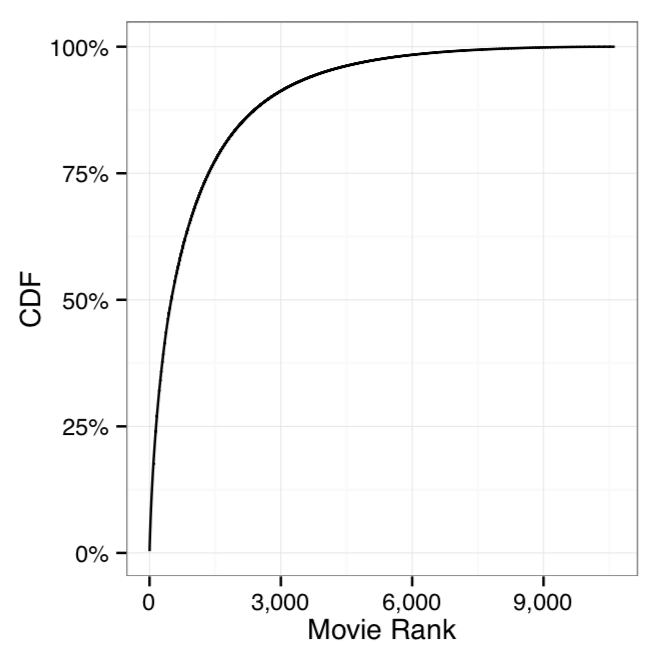
\includegraphics[width=0.4\linewidth]{figures/cdf.png}\\
Figure 2. The relationship between number of movie ratings and movie rank.
\end{center}
We also compute each user's eccentricity, or the median rank of each user's rated movies. Note that using the median makes the measure more robust to outliers. A bimodal distribution of eccentricity would suggest two different types of people, those with mainstream interests and those with niche interests. A unimodal distribution of eccentricity  would suggest that people generally have a mix of mainstream interests and niche interests. See Figure 3.
\begin{center}
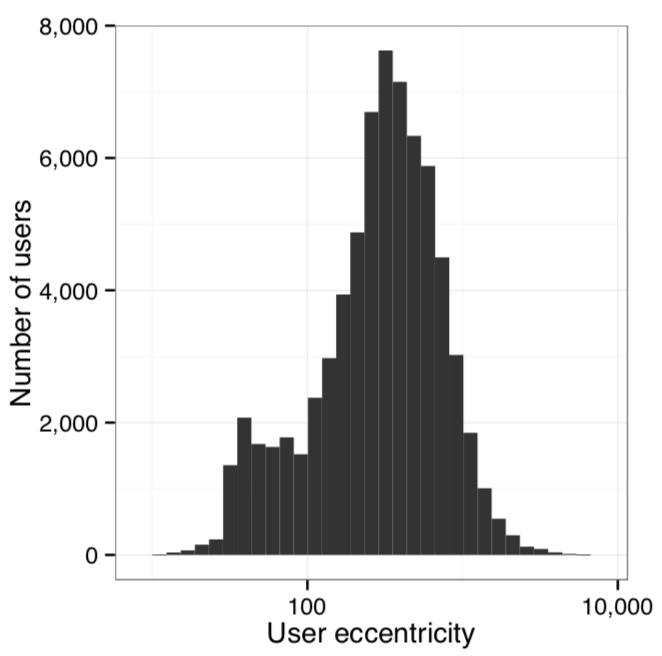
\includegraphics[width=0.4\linewidth]{figures/dist.png}\\
Figure 3. The distribution of user eccentricity.
\end{center}

\subsection{Group by operation}
The two charts below show the memory requirements for the group by operation under different scenarios. ``Distributions'' refers to whether we can store full histograms or not. ``Statistics'' refers to what kind of statistics we can compute. Let $N$ be the number of observations. Let $G$ be the number of distinct groups. Let $V$ be the largest number of distinct values within a group. See Tables 1 and 2. 
\begin{center}
\begin{tabular}{|c|c|c|c|}
\hline
Memory & Scenario                            & Distributions & Statistics \\
\hline
$N$    & Small dataset                       & Yes           & General    \\
$VG$   & Small distributions                 & Yes           & General    \\
$G$    & Small number of groups              & No            & Combinable \\
$V$    & Small number of outcomes            & No            & No         \\
$1$    & Large number of groups and outcomes & No            & No         \\
\hline
\end{tabular}\\
Table 1. Group by operation information for arbitrary input data.
\end{center}
\begin{center}
\begin{tabular}{|c|c|c|c|}
\hline
Memory & Scenario                            & Distributions & Statistics \\
\hline
$N$    & Small dataset                       & Yes           & General    \\
$VG$   & Small distributions                 & Yes           & General    \\
$G$    & Small number of groups              & No            & Combinable \\
$V$    & Small number of outcomes            & Yes           & General    \\
$1$    & Large number of groups and outcomes & No            & Combinable \\
\hline
\end{tabular}\\
Table 2. Group by operation information for pre-grouped input data.\\
\end{center}

\section{Demo}
\subsection{Command line tools}
Become familiar with basic command line tools using the tutorials on the ``Installing tools'' post on the course website. We saw examples of \textbf{ls}, \textbf{pwd}, \textbf{man}, \textbf{echo}, \textbf{touch}, \textbf{rm}, \textbf{cat}, \textbf{head}, \textbf{uniq}, \textbf{tr}, \textbf{cut}, \textbf{more}, and \textbf{less} to name a few. The \textbf{man} page for each command provides a guide for usage and various option flags. You should understand basic pattern matching, variable creation, variable referencing, and piping. Also be aware that single quote strings are interpreted literally and double quote strings are partially interpreted.
